%%%%%%%%%%%%%%%%%%%%%%%%%%%%%%%%%%%%%%%%%%%%%%%%%%%%%%%%%%%%%%%%%%%%%%%%%%
%% Review Volume (last updated on 2014/03/05) %%
%% Trim Size: 9.61in x 6.69in %%
%% Text Area: 8in (include runningheads) x 5in %%
%% Main Text: 10 on 13pt %%
%% For support: Yolande Koh, <ykoh@wspc.com.sg> %%
%% D. Rajesh Babu, <rajesh@wspc.com.sg> %%
%%%%%%%%%%%%%%%%%%%%%%%%%%%%%%%%%%%%%%%%%%%%%%%%%%%%%%%%%%%%%%%%%%%%%%%%%%
%%
%\documentclass[wsdraft]{ws-rv961x669} % to draw border line around text area
%\documentclass{ws-rv961x669}
\documentclass[addchapnum]{ws-rv961x669} % to add chapter number in volume
\usepackage{ws-rv-van} % numbered citation/references (default)
%\usepackage{ws-rv-thm} % comment this line when `amsthm / theorem / ntheorem` package is used
%\usepackage{subfigure} % required only when side-by-side / subfigures are used
\usepackage{ws-index} % required only when multiple indexes are used
%\usepackage[colorlinks=false]{hyperref}
%\usepackage{doi}
\usepackage{bbm}
\usepackage{amsmath}
\usepackage{amssymb}
\makeindex
\newindex{aindx}{adx}{and}{Author Index} % author index
\renewindex{default}{idx}{ind}{Subject Index} % subject index

% Useful macros for equations and units in HEP
\newcommand*{\bb}{\boldsymbol}
\newcommand{\req}[1]{Eq.~(\ref{#1})}
\newcommand{\rf}[1]{Figure~{\ref{#1}}}
\newcommand{\rt}[1]{Table~{\ref{#1}}}
\newcommand{\rsec}[1]{Section~{\ref{#1}}}
\newcommand{\rchap}[1]{Chapter~{\ref{#1}}}
\begin{document}

\chapter[Neutrinos in EM Fields]{Neutrinos in Electromagnetic Fields\label{JR_ch1}}

\author[J. Rafelski and A. Steinmetz]{Johann Rafelski and Andrew Steinmetz\footnote{JohannR@Arizona.EDU,AJSteinmetz@Arizona.EDU}}
\aindx{Rafelski, J.}
\aindx{Steinmetz, A.}

\address{Department of Physics, The University of Arizona, Tucson, AZ 85721, USA}

\begin{abstract}
Neutrino mixing is an important avenue for studying beyond standard model (BSM) physics as flavor mixing only occurs in the presence of massive neutrinos. However, as neutrinos are naturally massless in the standard model this presents a problem as there's no unique mechanism to introduce mass for neutrinos and it is yet unknown if neutrinos are Dirac-type or Majorana-type fermions. We establish that neutrino flavor mixing is not uniquely a property of mass, but also occurs from the possible magnetic dipole moment of the particles. We introduce a unified expressive for mass and magnetic moment and analyze how the PMNS rotation matrix may be sensitive to strong electromagnetic fields.
\end{abstract}

\markboth{Johann Rafelski and Andrew Steinmetz}{Neutrinos in EM fields} % Customized running heads

\body

%\tableofcontents\

%%%%%%%%%%%%%%%%%%%%%%%%%%%%%%%%%%%%
\section{Introduction}
\label{sec:intro}
%%%%%%%%%%%%%%%%%%%%%%%%%%%%%%%%%%%%
\noindent Neutrinos are among the most abundant particles in the universe. Despite their difficult to measure effects today, neutrinos once were the dominant form of energy density in the universe~\cite{Rafelski:2023emw} and still play an important role in the deaths of stars today. Therefore it is of interest to study their electromagnetic properties in strong field conditions.

The size of the neutrino magnetic dipole moment is relatively small with a lower bound determined by the standard model and an upper bound from reactor or solar observations given by~\citep{Studenikin:2016ykv,Canas:2015yoa,AristizabalSierra:2021fuc}

\begin{align}
    \label{momentbound:1}
    10^{-19}\mu_{B}<\mu_{\nu}^\mathrm{eff}<10^{-10}\mu_{B}\,,\qquad\mu_{B}=\frac{e\hbar}{2m}
\end{align}

where $\mu_{B}$ is the Bohr magneton and $\mu_{\nu}^\mathrm{eff}$ is the effective and characteristic size of the neutrino magnetic moment. In the standard model, neutrinos do not interact electromagnetically at tree level as they are only coupled to the weak interaction via the $SU(2)_{L}$ doublet~\citep{Schwartz:2014sze}.

However, through higher order loop interactions it is expected that the neutrino should manifestation some non-minimal EM interactions~\citep{Shrock:1980vy,DUNE:2020fgq} of the form
\begin{gather}
    \bb{\mu_{\nu}}=
	\begin{pmatrix}
		\mu_{ee} & \mu_{e\mu} & \mu_{e\tau} \\
		\mu_{e\mu}^{*} & \mu_{\mu\mu} & \mu_{\mu\tau} \\
		\mu_{e\tau}^{*} & \mu_{\mu\tau}^{*} & \mu_{\tau\tau}
	\end{pmatrix}
\end{gather}
This leaves open the possibility for Beyond Standard Model (BSM) physics to produce an abnormally large electromagnetic dipole~\citep{Giunti:2014ixa,Lindner:2017uvt,Brdar:2020quo} between the bounds of~\req{momentbound:1} which may manifest in strong field or matter dense environments.

%%%%%%%%%%%%%%%%%%%%%%%%%%%%%%%%%%%%%%%
\subsection{Status of neutrino flavor mixing}
\label{sec:numass}
%%%%%%%%%%%%%%%%%%%%%%%%%%%%%%%%%%%%%%%
\noindent As neutrinos have masses, there is no guarantee that their $SU(2)_{L}$ flavor eigenstates will be simultaneously their propagating mass eigenstates. This misalignment between the two representations can then written as rotation of the neutrino flavor 3-vector where $N=3$ is the number of generations. The unitary mixing matrix $\bb{V}$ allows for the change of basis between mass and flavor eigenstates via
\begin{alignat}{1}
	\label{basis:1} \bb{\nu_{f}}=\bb{V}\bb{\nu_{m}}\,\rightarrow
	\begin{pmatrix}
		\nu_{e}\\
		\nu_{\mu}\\
		\nu_{\tau}
	\end{pmatrix}=
	\begin{pmatrix}
		V_{e1} & V_{e2} & V_{e3}\\
		V_{\mu1} & V_{\mu2} & V_{\mu3}\\
		V_{\tau1} & V_{\tau2} & V_{\tau3}
	\end{pmatrix}
	\begin{pmatrix}
		\nu_{1}\\
		\nu_{2}\\
		\nu_{3}
	\end{pmatrix}\,,
\end{alignat}
where $\bb{\nu_{f}}$ is the neutrino state vector written in the flavor basis while $\bb{\nu_{m}}$ is written in the mass basis. Boldface type will be used for matrices and vectors. Bars atop vectors represent the Dirac adjoint in the usual manner.

The mixing matrix's form then depends on the Dirac-like or Majorana-like nature of the neutrinos
\begin{alignat}{1}
	\label{phases:1} &\bb{V} = \bb{U}\bb{P}\,,\\
	\label{phases:2} &\bb{P}_\mathrm{Dirac} = \mathbbm{1}\,,\\
	\label{phases:3} &\bb{P}_\mathrm{Maj.} = \mathrm{diag}(e^{i\rho},e^{i\sigma},1)\,.
\end{alignat}
Majorana neutrinos allow up to two additional complex phases $\rho$ and $\sigma$ which participate in CPV. In the standard parameterization~\citep{Schwartz:2014sze}, the rotation matrix $\bb{U}$ can be expressed as
\begin{alignat}{1}
	\label{rotation:1} \bb{U} =
	  \begin{pmatrix}
		  c_{12}c_{13} & s_{12}c_{13} & s_{13}e^{-i\delta}\\
		  -s_{12}c_{23} - c_{12}s_{13}s_{23}e^{i\delta} & c_{12}c_{23} - s_{12}s_{13}s_{23}e^{i\delta} & c_{13}s_{23}\\
		  s_{12}s_{23} - c_{12}s_{13}c_{23}e^{i\delta}& -c_{12}s_{23} - s_{12}s_{13}c_{23}e^{i\delta} & c_{13}c_{23}
	  \end{pmatrix}\,,
\end{alignat}
where $c_{ij} = \mathrm{cos}(\theta_{ij})$ and $s_{ij} = \mathrm{sin}(\theta_{ij})$. In this convention, the three mixing angles $(\theta_{12}, \theta_{13}, \theta_{23})$, are understood to be the Euler angles for generalized rotations. There are many possible parametrizations for the mixing matrix and without a working model of the underlying physics, they represent generic observables which are otherwise not predicted. Another relevant choice is the~\cite{wolfenstein1983parametrization} parameterization, but as neutrinos mixing angles are rather large unlike the parameters for the CKM matrix in the quark sector, we will not use it here.

The Majorana mass Lagrangian in the flavor basis can then be written as
\begin{alignat}{1}
	\label{mass:1} -\mathcal{L}_{\mathrm{mass}}^{\mathrm{Maj.}}&=\frac{1}{2}\bb{\bar{\nu}_{f}^{L}}\bb{M}_{\nu}\left(\bb{\nu_{f}^{L}}\right)^{c}+\mathrm{h.c}\,,
\end{alignat}
where $\bb{\nu^{L}}$ refers to left-handed chiral states which can be obtained using projection operators and $\gamma^{5}$. The superscript $\bb{\nu}^{c}$ refers to the charge conjugated state where $\bb{\nu}^{c} = \hat{C}(\bb{\bar{\nu}})^\mathrm{T}$ is the charge conjugate of the neutrino field. The operator $\hat{C} = i\gamma^{2}\gamma^{0}$ is the charge conjugation operator which can be written as a $4\times4$ matrix for a given representation as each flavor is in this formulation a four-component spinor.


%%%%%%%%%%%%%%%%%%%%%%%%%%%%%%%%%%%%
\section*{Acknowledgements}
Harald Fritzsch enjoyed the US-South-West. On the way between Caltech and the Santa Fe Institute he sometimes made a stop at the half-way point, Tucson. On such occasions he explored Arizona mountains and  deserts; Figure\,\ref{Fig:AZcolloq2007} is showing our outing on occasion of March 23, 2007 physics colloquium at the University of Arizona: Harald was an avid observer and photographer of the desert fauna and flora. 
 
\begin{figure}%[hb]
\centerline{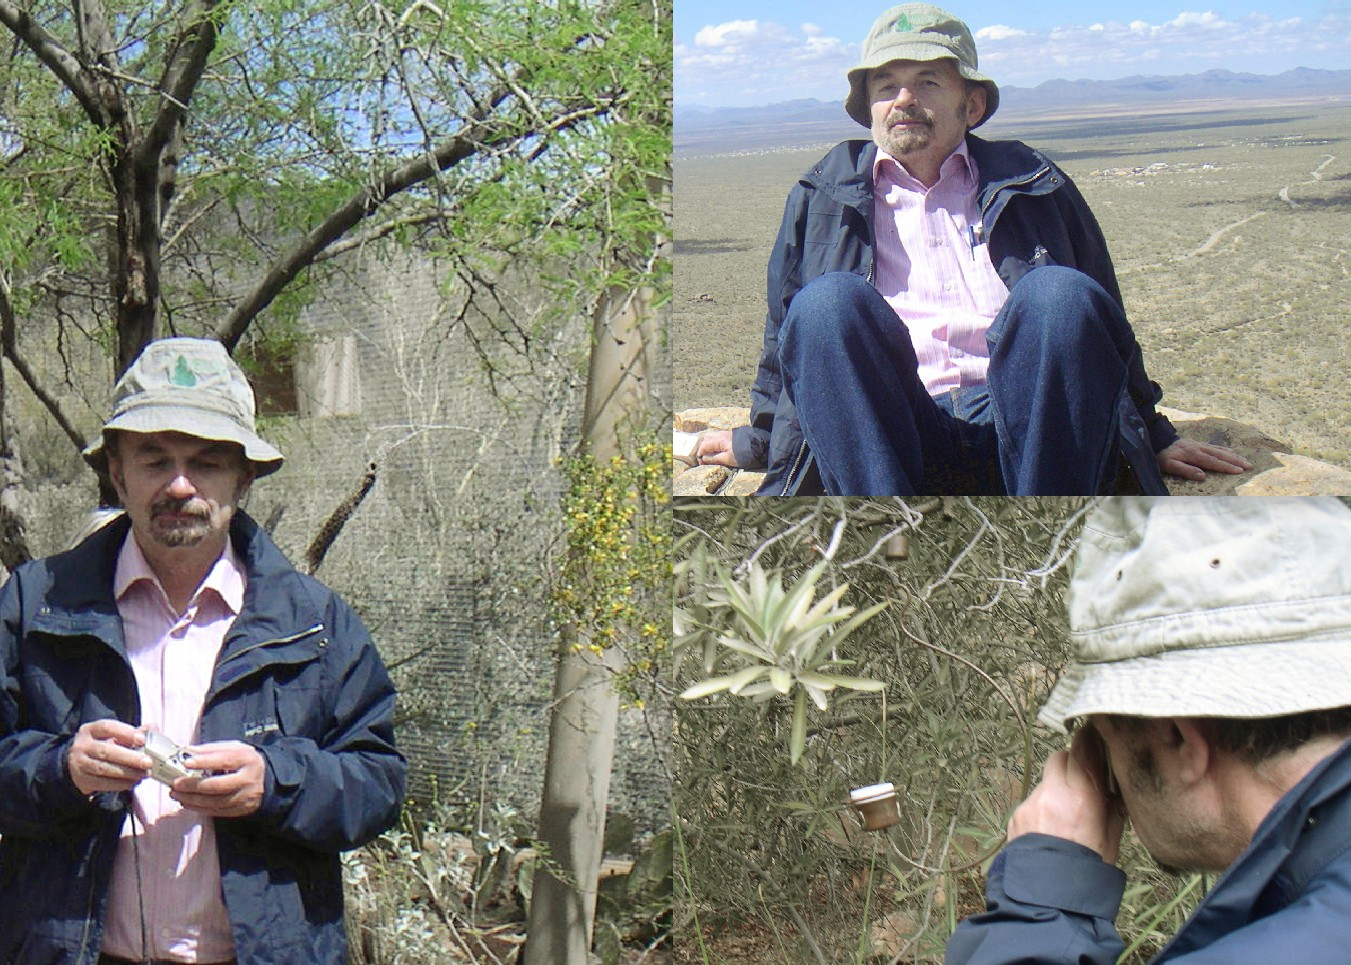
\includegraphics[width=0.95\columnwidth]{07March24HaraldCollageDesertMuseum.jpg}}
\caption{Harald Fritzsch visiting Arizona-Sonora Desert Museum in Spring 2007. Pictures and picture assembly by Johann Rafelski
}
\label{Fig:AZcolloq2007} 
\end{figure}

These meetings offered an opportunity to exchange ideas the  origin of neutrino mass and parameters of  the standard model were close to his heart. Were these parameters really natural constants on cosmological time scale? In Figure\,\ref{Fig:RANP2004} we see Harald's first transparency ``Time Dependence of QCD and Experimental Tests'' made at at the 9th Hadron Physics and 7th Relativistic Aspects of Nuclear Physics (HADRON-RANP 2004): A Joint Meeting on QCD and QGP: Rio de Janeiro, Brazil, March 28-April 3, 2004~\cite{Fritzsch:2004civ}, a meeting we both attended. We see that Harald modified slightly by hand the typed transparency to introduce the meeting specific context in a talk which arose from another publication of the epoch, Ref.\,\cite{Calmet:2001nu}. 

\begin{figure}%[ht]
\centerline{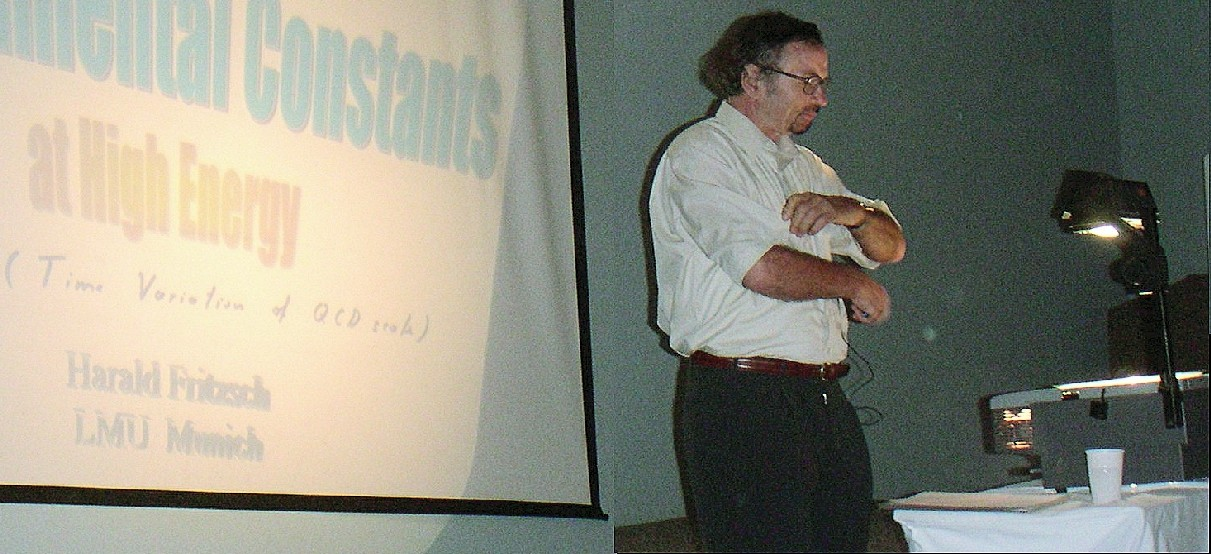
\includegraphics[width=0.95\columnwidth]{04RANPHarald1Ed.jpg}}
\caption{Harald begins his presentation in Rio de Janeiro 2004 about time dependence of QCD, see text for details. Picture by Johann Rafelski
}
\label{Fig:RANP2004} 
\end{figure}
 
%%%%%%%%%%%%%%%%%%%%%%%%%%%%%%%%%%%%


\bibliographystyle{ws-rv-van}
\bibliography{Rafelski_Steinmetz_for_Harald}
%%%%%%%%%%%%%%%%%%%%%%%%%%%%%%%%%%%%
\end{document} 
%%%%%%%%%%%%%%%%%%%%%%%%%%%%%%%%%%%%
